\section{Holiday and Sick Leave Detection}

Figure~\ref{fig:missing-time} shows the analysis of the author for his work repositories.
The y-axis shows the additions or deletions of commits, the x-axis shows the week of a year.
For better verification and evaluation of the results, a scatter plot with the additions and deletions for each commit has been added on top of the miss-out graph.

The evaluation of this algorithm turned out to be quite difficult, as there is no publicly available information about sick leave or holiday.
For the purpose of this thesis I had to use anonymous statistics of several friends and colleagues to evaluate the algorithm.
The algorithm successfully manages to find all anomalies, which occurred in the last year, for all seven regarded users.

A not intended side effect of detecting prototypes is that the algorithm not only detected anomalies, such as sick leave or holiday, but also also found inconsistencies in the work routine.
For instance between week 37 to 45 in Figure~\ref{fig:missing-time} I was forced to reduce my working hours due to legal questions and continuously shift hours and working days for several weeks.
It is hard to interpret those inconsistencies without more contextual information, but nevertheless it provides the fact that something happened during this time.

\begin{figure}[H]
    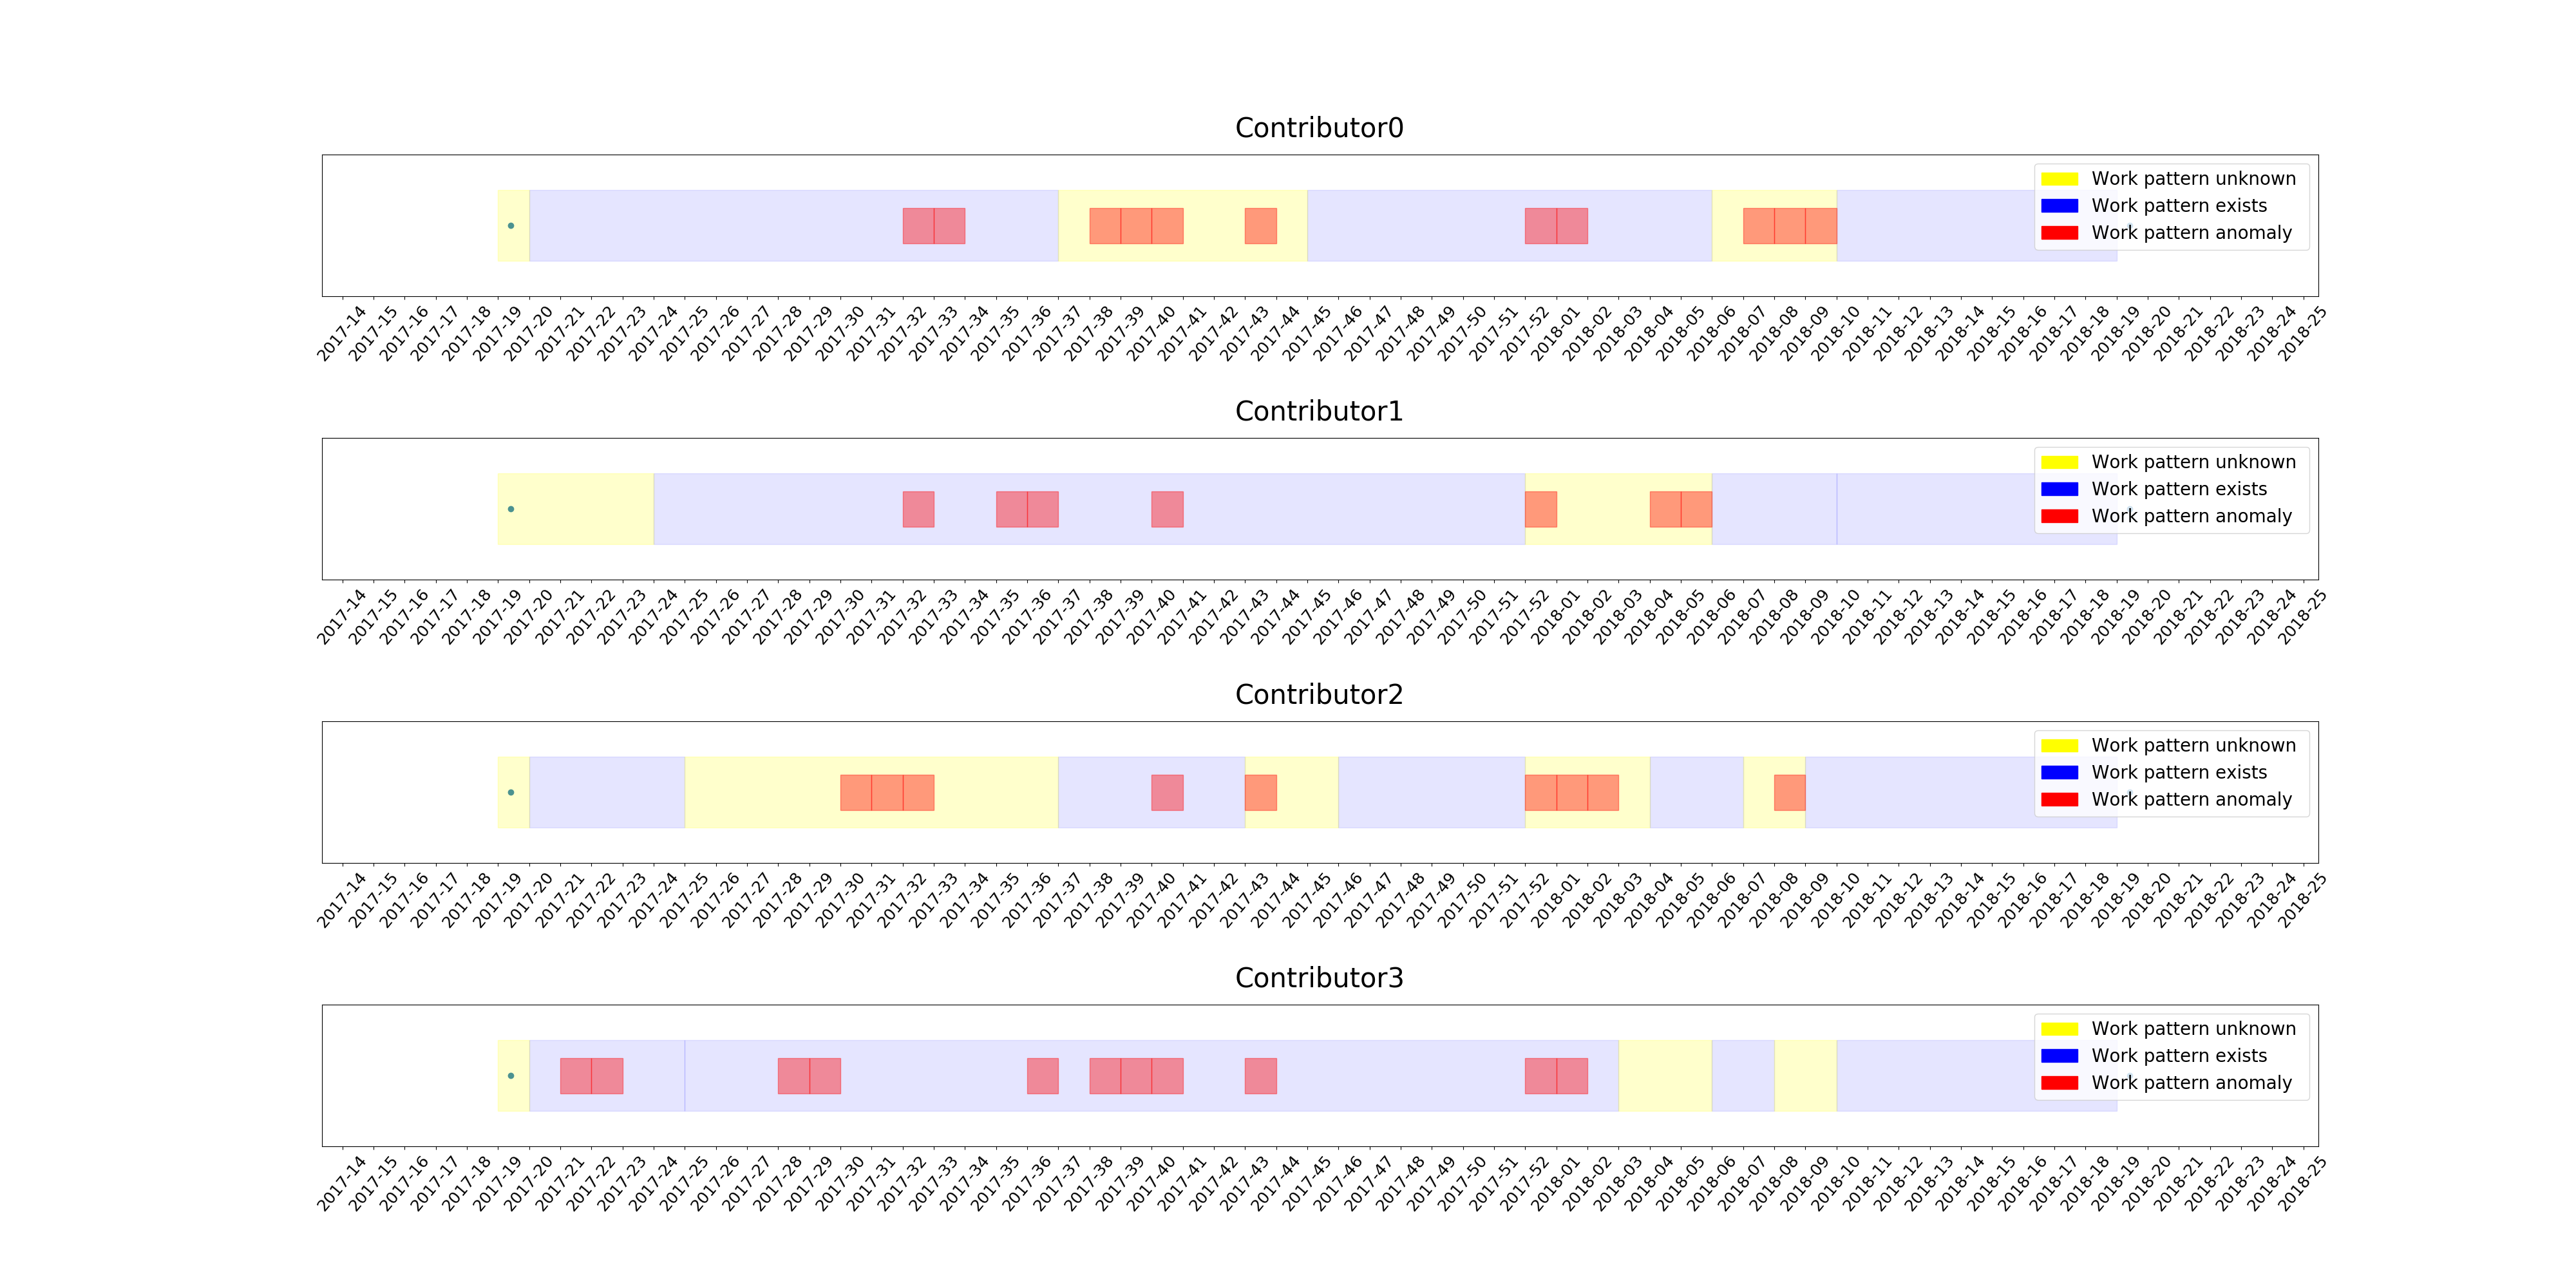
\includegraphics[scale=0.20]{./graphs/analysis/work-time-analysis-comparison}
    \centering
    \caption{The miss-out analysis graphs of four employees.}\label{fig:miss-out-comparison}
\end{figure}

In Figure~\ref{fig:miss-out-comparison} the comparison between multiple employees can be seen.
\emph{Contributor0} and \emph{Contributor2} are working on flexible work time, which reflects in the inconsistencies in the work patterns (yellow sections in ~\ref{fig:miss-out-comparison}) of those contributors.
The other two contributors have very consistent working hours patterns, as can be seen by the long lasting blue sections.
